\subsection{Apporter des modifications au code source}
\existstill{1.0.0}

Une fois que vous accédez au code source de l'application, vous pouvez en faire ce que vous voulez.
Si participer à l'évolution vous intéresse, vous êtes encouragé à me faire des pull requests que je mergerais dans le dépôt principal si votre travail répond correctement à un ticket ayant l'état \emph{accepté}.

N'ayant jamais effectué ce genre d'actions pour le moment, je ne suis pas sûr qu'il s'agisse de la meilleure façon de faire, ni même qu'elle soit réellement pratique sur le long terme, mais on aura toujours l'occasion de changer ça une fois ce logiciel massivement maintenu \Winkey.

\subsubsection{Convention de code}
\existstill{1.0.0}

Dans un souci de cohérence, de brèves consignes de style ont été mises en place. Il vous est demandé de les respecter~:
\begin{itemize}
	\item Les commentaires ainsi que les variables doivent être écrits en anglais.
	\item On utilise le \emph{snake\_case}.
	\item Une tabulation est employée pour l'indentation.
	\item Deux espaces sont insérés pour les brisements de lignes.
	\item La virgule touche touche toujours un caractère à gauche, et possède un espace ou un saut de ligne à droite.
	\item On ne saute pas de ligne avant l'accolade ouvrante.
	\item Une parenthèse, accolade ou crochet fermant doit être au même niveau d'indentation que son binôme ouvrant.
\end{itemize}

Le listing~\ref{fig_3.1_conventions} est un exemple permettant d'illustrer l'histoire de l'indentation et du brisement de lignes.
Les boules grises représentent des espaces, et les flèches une tabulation.

\begin{lstlisting}[basicstyle=\normalsize, caption={Conventions de code}, label=fig_3.1_conventions]
sub write_stuff(
~{\color{gray}$\bullet\bullet$}~$param_one,
~{\color{gray}$\bullet\bullet$}~$param_two
) {
~{\color{gray}--->}~print "$param_one $param_two";
}
\end{lstlisting}

\subsubsection{Workflow \emph{Git}}

\existstill{1.0.0}
\paragraph{Les types de branches}
La figure~\ref{fig_3.2_git} (qui est moche pour le moment, mais sera refaite avec \emph{TikZ} un jour) illustre de façon plus visuelle les explications ci-dessous.
Notez qu'il manque néanmoins la branche \emph{master} et les branches \emph{release} sur celle-ci, elle n'est donc pas tout à fait juste non plus\dots

Attention, pour le moment il s'agit d'un workflow plutôt théorique et qui reste très confus\dots
Je n'ai en effet pas encore eu l'occasion de le mettre en pratique. Celui-ci est susceptible de changer~!

\begin{description}
	\item[Branche \emph{master}]
		Elle pointera toujours sur la dernière version stable.
		Même si cela nécessite un changement de version majeure.
	\item[Branche \emph{development}]
		C'est sur celle-ci qu'on mergera les tickets relatifs à la prochaine version mineure ou majeure en cours de développement.
		Quand ceux-ci sont terminés, une nouvelle branche stable sera créée depuis celle-ci, ainsi que la branche \emph{bugfixes} correspondante.
	\item[Branches stables]
		Une branche est créée pour chaque version majeure et mineure du logiciel. Ces branches doivent être utilisées en production.
	\item[Branches bugfixes]
		Permettent la préparation des correctifs.
		Une branche \emph{bugfixes} n'existe qu'avant la publication d'une nouvelle version de correctifs.
		Quand nous estimons que celle-ci contient suffisamment d'éléments pour justifier une release, elle sera mergée sur la branche stable correspondante, incrémentant ainsi le numéro \emph{z} de la version.
		La branche pourra ensuite être supprimée et recrée à partir de la nouvelle version mineure si besoin est.
	\item[Branches d'implémentations]
		Une branche d'implémentation doit être créée pour chaque ticket.
		La base de cette branche dépendra du type de ticket, on en parle dans un paragraphe sous-jacent.
		Une fois les développements réalisés et mergés au bon endroit, nous pouvons supprimer la branche pour éviter de polluer le git.
		Deux types de branches d'implémentation existent~:
		\begin{description}
			\item[Implémentation de fonctionnalités]
				Elles partent de l'état courant de \emph{master} et sont à utiliser pour l'accomplissement d'un ticket d'évolution.
				Une fois le développement considéré comme terminé, la branche pourra être mergée dans \emph{developement}.
				Si après ce merge, on s'aperçoit d'un bug ou d'une régression entrainée par celui-ci, il faudra continuer à publier les correctifs sur cette branche, puis la remerger dans \emph{development}.
				Attention à bien la conserver jusqu'à ce qu'elle soit mergée sur une branche stable.
			\item[Implémentation de correctifs]
				Ces branches partent de la première version stable ayant le problème.
				Elles seront ensuite mergées dans les branches \emph{bugfixes} de chaque autre version touché par l'anomalie, voir dans \emph{development} si elle monte aussi haut.
				Idéalement, le correctif devrait donc se présenter sous la forme d'un seul commit, ce qui rend facile le \emph{cherry-pick}.
		\end{description}
\end{description}

\paragraph{Procédure de merge}
De façon générale, les messages de commit doivent être écrits en anglais. \emph{Git} doit aussi être correctement configuré pour que le nom et l'adresse email de l'utilisateur soient les bons.
Une fois une branche de développement prête à être mergée, le commit devra avoir un message dont la première ligne ressemble à~:\\
{\tt[<signe\_ticket>] \#<numéro\_ticket>: <description>.}\\
Avec~:
\begin{itemize}
	\item\emph{<description>} -- dois commencer par une minuscule, et décrire de façon concise ce qui a été réalisé dans le commit.
	\item\emph{<signe\_ticket>} -- le signe du ticket dépend grandement du type de branche sur laquelle nous sommes.
\end{itemize}
Si le message de commit mérite de plus amples informations, on pourra marquer ce texte après un saut de ligne.
	Le signe du ticket peut ici avoir trois états différents~:
		\begin{itemize}
			\item {\tt+} en cas de traitement d'une évolution.
			\item {\tt-} en cas de correction d'anomalie publiée.
			\item {\tt*} en cas de correction d'anomalie d'évolution (évolution déjà mergée dans \emph{development} mais qui nécessite un nouveau merge à cause d'une régression).
		\end{itemize}
Voici des indications plus précises concernant les branches en fonction de leurs types~:
\begin{description}
	\item[Branches d'implémentations]
		N'oubliez pas qu'il s'agit là des seules branches pouvant réellement avoir du contenu applicatif.
		Les commits peuvent ici avoir une forme assez libre. Comme d'habitude, privilégiez d'en faire de petits, ayant des messages précis sur leurs apports. \item[Branche \emph{development}]
		Une fois une fonctionnalité mature, elle peut être mergée sur \emph{development}.
		À ce moment, la branche d'implémentation en question ne doit pas être supprimée, car le pointeur sera nécessaire pour merger une seconde fois sur une branche stable.
		Notez que ce merge doit être fait avec l'option \emph{--no-ff} pour éviter de n'avoir qu'un simple déplacement de pointeur au niveau de \emph{Git}.\\

		Le message de ce commit peut avoir la forme générique présentée ci-dessus, avec un {\tt+} ou {\tt*} comme signe de ticket.
	\item[Branches de release et branches stables] 
		Une fois des développements suffisamment testés (sur la branche \emph{development}), une nouvelle version pourra être publiée incluant toutes les évolutions validées.
		Il s'agira d'une incrémentation de version mineure si la rétrocompatibilité n'est pas brisée, ou sinon de la version majeure.
		Dans ce premier cas, n'oubliez pas d'également merger la nouvelle branche dans la version majeure concernée.\\

		Concrètement parlant, on créera ici une nouvelle branche depuis une branche stable que l'on veut voir évoluer (une branche majeure ou mineur) qui s'appellera \emph{release-vx.y.0}.
		Sur cette branche nous mergerons toutes les branches d'implémentations que l'on désire inclure dans cette nouvelle version.
		Finalement, on créera un nouveau commit (vide ? (option \emph{allow-empty})) à la tête de celle-ci, ayant comme première ligne sur le message de commit~:
		{\tt[RELEASE] vx.y.0}
		Avec \emph{x} et \emph{y} qui représente le nouveau numéro de version (\emph{z} sera forcément à zéro).
		Les autres lignes peuvent être un rapide journal des changements présentant les différents tickets intégrés à l'évolution.\\
		Si le package ainsi produit fonctionne bien, la release sera validée, et un merge avec l'option \path{no-ff} sur la branche stable pourra être effectué.
		Nous pouvons finalement supprimer la branche de release.

		Depuis ce commit, un tag sera créé avec le même numéro de version(\path{git tag -m x.y.0 -a x.y.0}), mais sans le préfixe \emph{v}.
	\item[Branches bugfixes]
		Une branche \emph{bugfixes} devra être créée en parallèle de chaque version stable.
		Elle se chargera d'agréger les branches d'implémentation correspondant à des corrections à intégrer.
		Le changelog ne devra présenter que les correctifs publiés.
		Notons qu'il ne devrait de toute façon rien avoir d'autre de modifié.\\

		Quand la branche \emph{bugfixes} est freezée, elle sera mergée avec comme message de commit {\tt[RELEASE] vx.y.z} dans la branche stable à laquelle elle est liée.
		À présent, cette branche \emph{bugfixes} pourra être supprimée et pourra être recréée depuis cette nouvelle version stable pour accueillir les futurs correctifs.
\end{description}

\begin{figure}
	\centering
	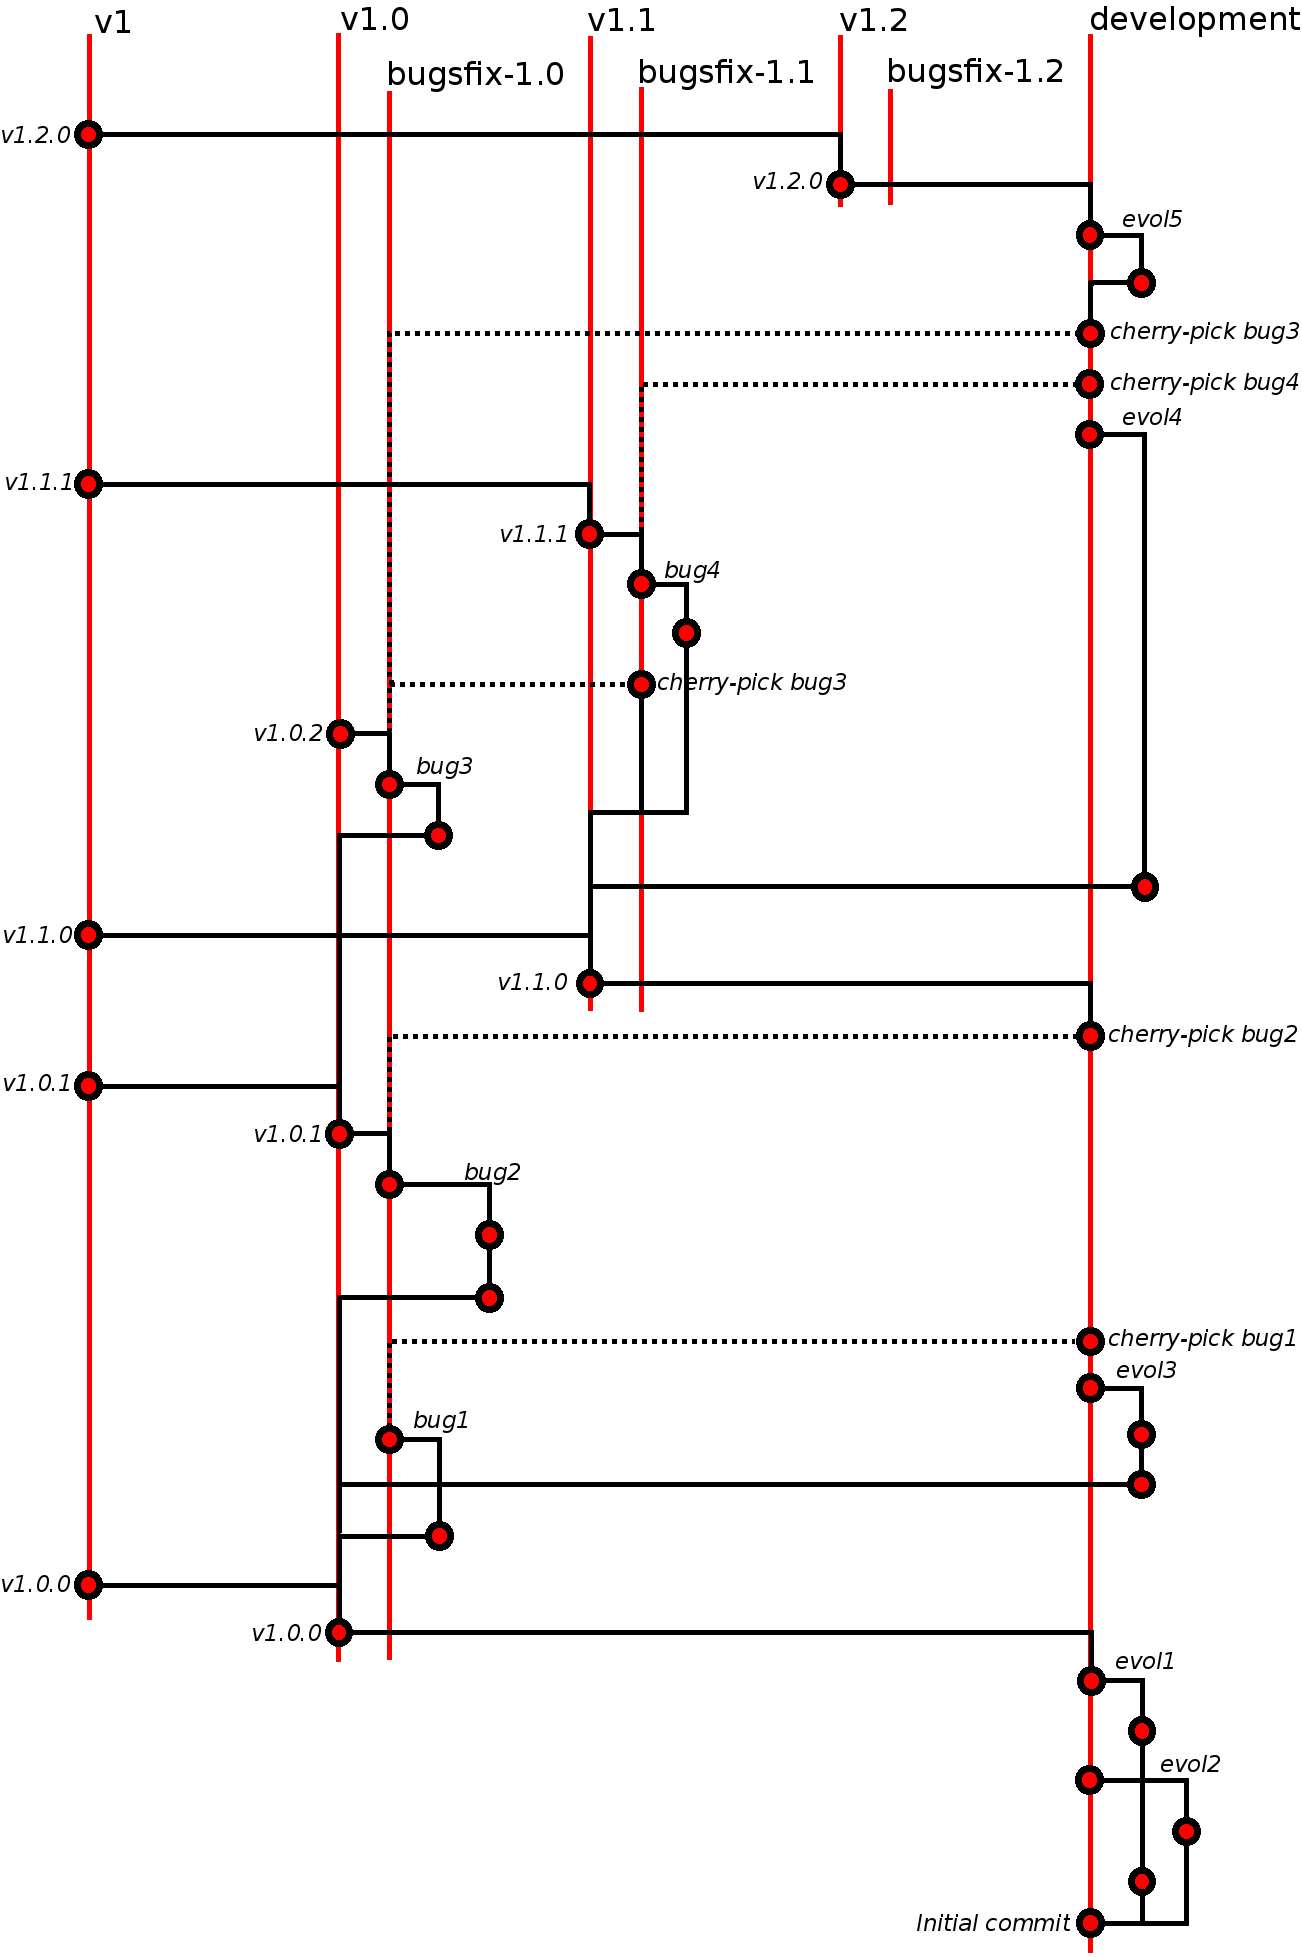
\includegraphics[scale=0.3]{part/developpement/code/fig_workflow_git.png}
	\caption{Workflow git}
	\label{fig_3.2_git}
\end{figure}

\subsubsection{Publier une nouvelle release}

\existstill{1.0.3}
Quand un ticket est considéré comme implémenté, il peut être mergé sur la branche \path{preparation-vx.x.x}, permettant ainsi sa propulsion dans une version future.
Si tous les tickets prévus pour la release sont implémentés et fonctionnels, voici la procédure à établir pour la livrason d'une nouvelle version~:

\begin{itemize}
	\item Jouer les tests d'intégration sur la branche de préparation et valider que tout se passe bien.
	\item Utiliser le script \path{dev/version_updater.pl} pour mettre à jour tous les numéros de version présents un peu partout dans le code source. Commitez le résultat directement sur la branche de préparation.
	\item Mettre en place le tag correspondant à la version publiée sur le commit de mise à jour du numéro de version.
	\item Si necessaire, mergez cette branche dans la branche suivant les évolutions de la version majeure et/ou mineur dont la version publiée appartient.
\end{itemize}
